\documentclass[11pt]{article}
\usepackage[latin1]{inputenc}
\usepackage{amsmath}	%math stuff
\usepackage{amsfonts}	
\usepackage{amssymb}	

\usepackage{graphicx}	%insert graphics
\usepackage{microtype}	%improves spacing
\usepackage{float}		%H postion	
\usepackage{caption}	%caption w/o : 	
\usepackage{framed}		%creates frames
\usepackage{enumitem}

%\usepackage{listings}	%insert sourcecode
\usepackage{color}
\usepackage{pdfpages}	%include PDF pages

\usepackage{bigstrut}	%exce2latex table packages
\usepackage{rotating}
\usepackage{multirow}
\usepackage{booktabs}

\usepackage{cleveref}	%cooler references, needs to be last

\usepackage[margin=1.0in]{geometry}	%for some reason, looks beter. 
\geometry{a4paper}

\usepackage[framed]{mcode}
\graphicspath{{../Figures/}{../figures/}}

\usepackage{fancyhdr}
\pagestyle{fancy}
\lhead{ECE 3522}
\rhead{Berezowsky \thepage}
\cfoot{}

\usepackage[bookmarks]{hyperref}

\title{Computer Assignment 01: Simple Statistics}
\author{Tyler Berezowsky}

\begin{document}
\maketitle
\section{Problem Statement} 
%Summarize the problem statement in one paragraph. Clearly state what the knowns are and what unknowns you must find
The purpose of this assignment was to develop proficiency loading and processing various types of time series data in MATLAB. Specifically, an audio signal and a stock price trend were loaded and processed. Processing consisted of calculating global statistics (minimum, maximum, mean, median, and variance), filtering the signal via the frame and window approach, and recalculating mean and variance for each window. 
\section{Approach and Results} 
%Describe your approach to finding the unknowns. Use numbered figures, tables and equations where necessary.
\subsection{The Signal Abstraction} 
While a Google stock trend and an audio signal qualitatively are completely separate identities, quantitatively they are described the same. Both are time dependent signals described by sample points of varying amplitude values and indexed by either the sample rate or a time vector. Therefore, once the signal is translated into a matrix or vector, the procedure for processing is identical in MATLAB. 


The Google stock data set contained five vectors; the stock's opening price, closing price, minimum price, peak price and the date at which the data was collected. It is assumed the date is independent and all other vectors are dependent. The data was delivered through an excel spreadsheet. 


The audio data set consisted of a single vector. The points were plotted in time by generating a time vector based on the sample rate of the audio signal. The data was deliver through a .raw file consisting of 16 bit signed integers for each sample point. 


\subsection{Loading the Data Set}
The Google stock data was loaded via the \verb|xlsread| command. The command transferrs each column of a spreadsheet into a vector of a matrix.

The audio signal was transfer to MATLAB through the command \verb|fread| which places the sample points in the .raw file into a vector.

\subsection{Plotting} 
 The entire Google stock data set was plotted utilizing the \verb|highlow| command which plots a vertical bar that spans the high and low prices of the stocks value on a specific day. In addition, tick marks are plotted on the bar representing the opening and closing prices. The plot's abscissa is time given as dates. The closing price of the stock and date was also plotted as requested. The plots are displayed in figure~\ref{fig: plot_01}.

\begin{figure}[H] %plot of google signal 
	\centering 
	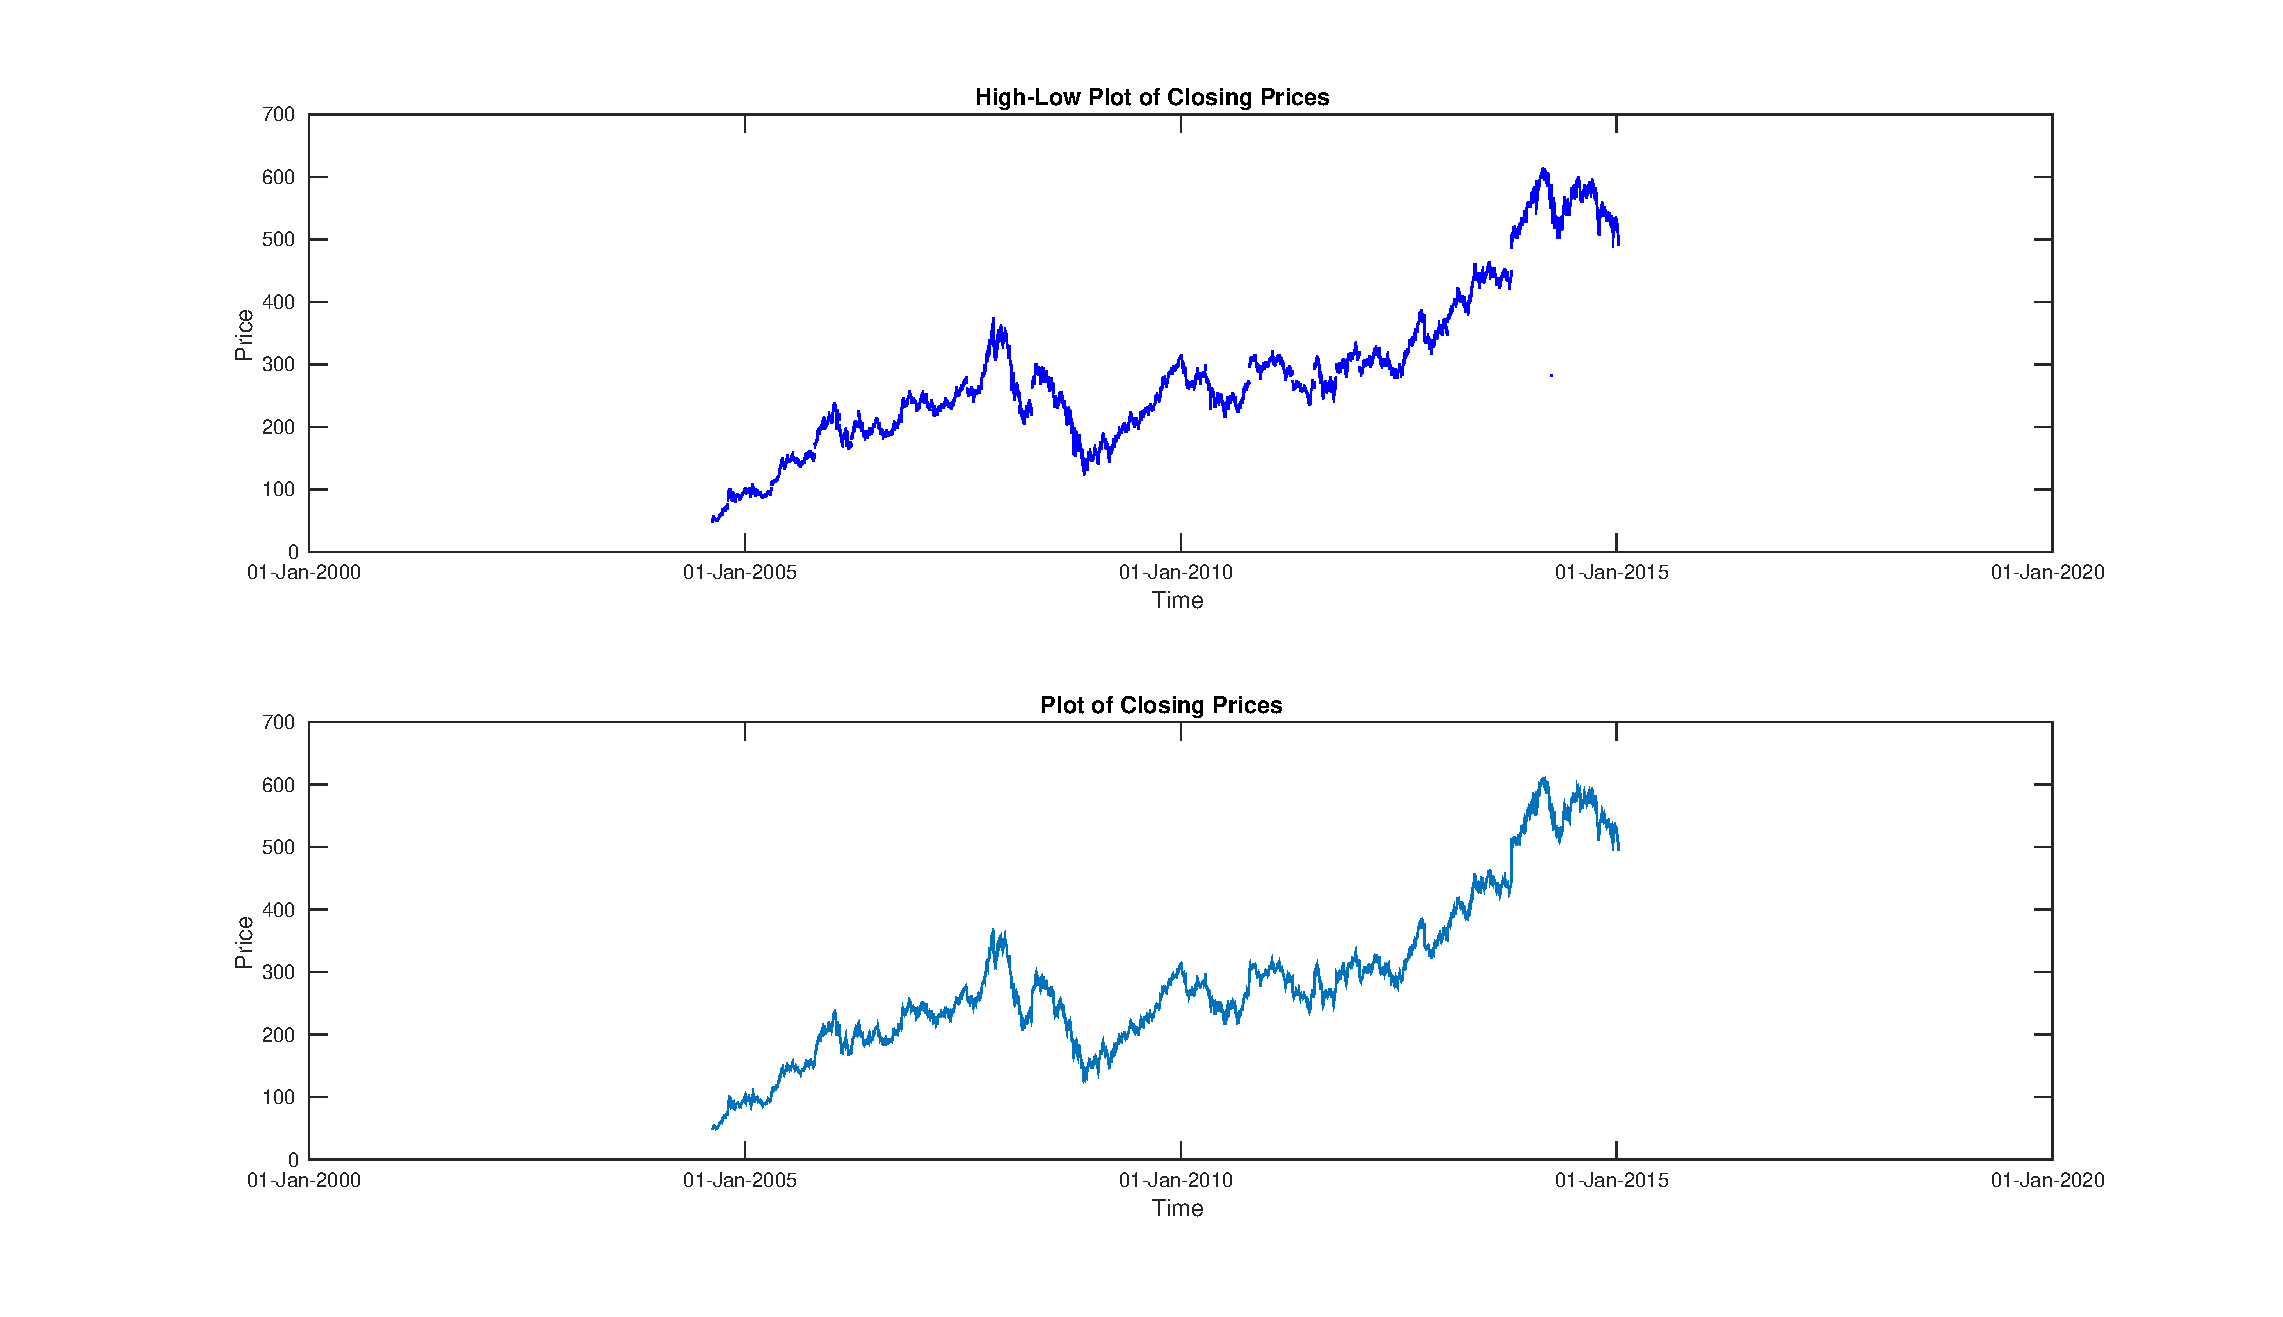
\includegraphics[width=\linewidth]{plot_01}
	\caption{Plot of Google stock prices via a ``High-Low'' plot with displays the range of prices for each day, and a normal plot.}
	\label{fig: plot_01} 
\end{figure}

The overall trend of the stock for both plots is identical. The \verb|highlow| plot appears nosier due its data points representing the range of the stock price for a day instead of a single point. 

Plotting the audio signal was identical to plotting the closing stock prices. A time vector was calculated for the signal utilizing the sample rate and the number of samples in the signal. The plot can be seen in figure~\ref{fig: plot_03}. 

\begin{figure}[H] %audio signal 
	\centering 
	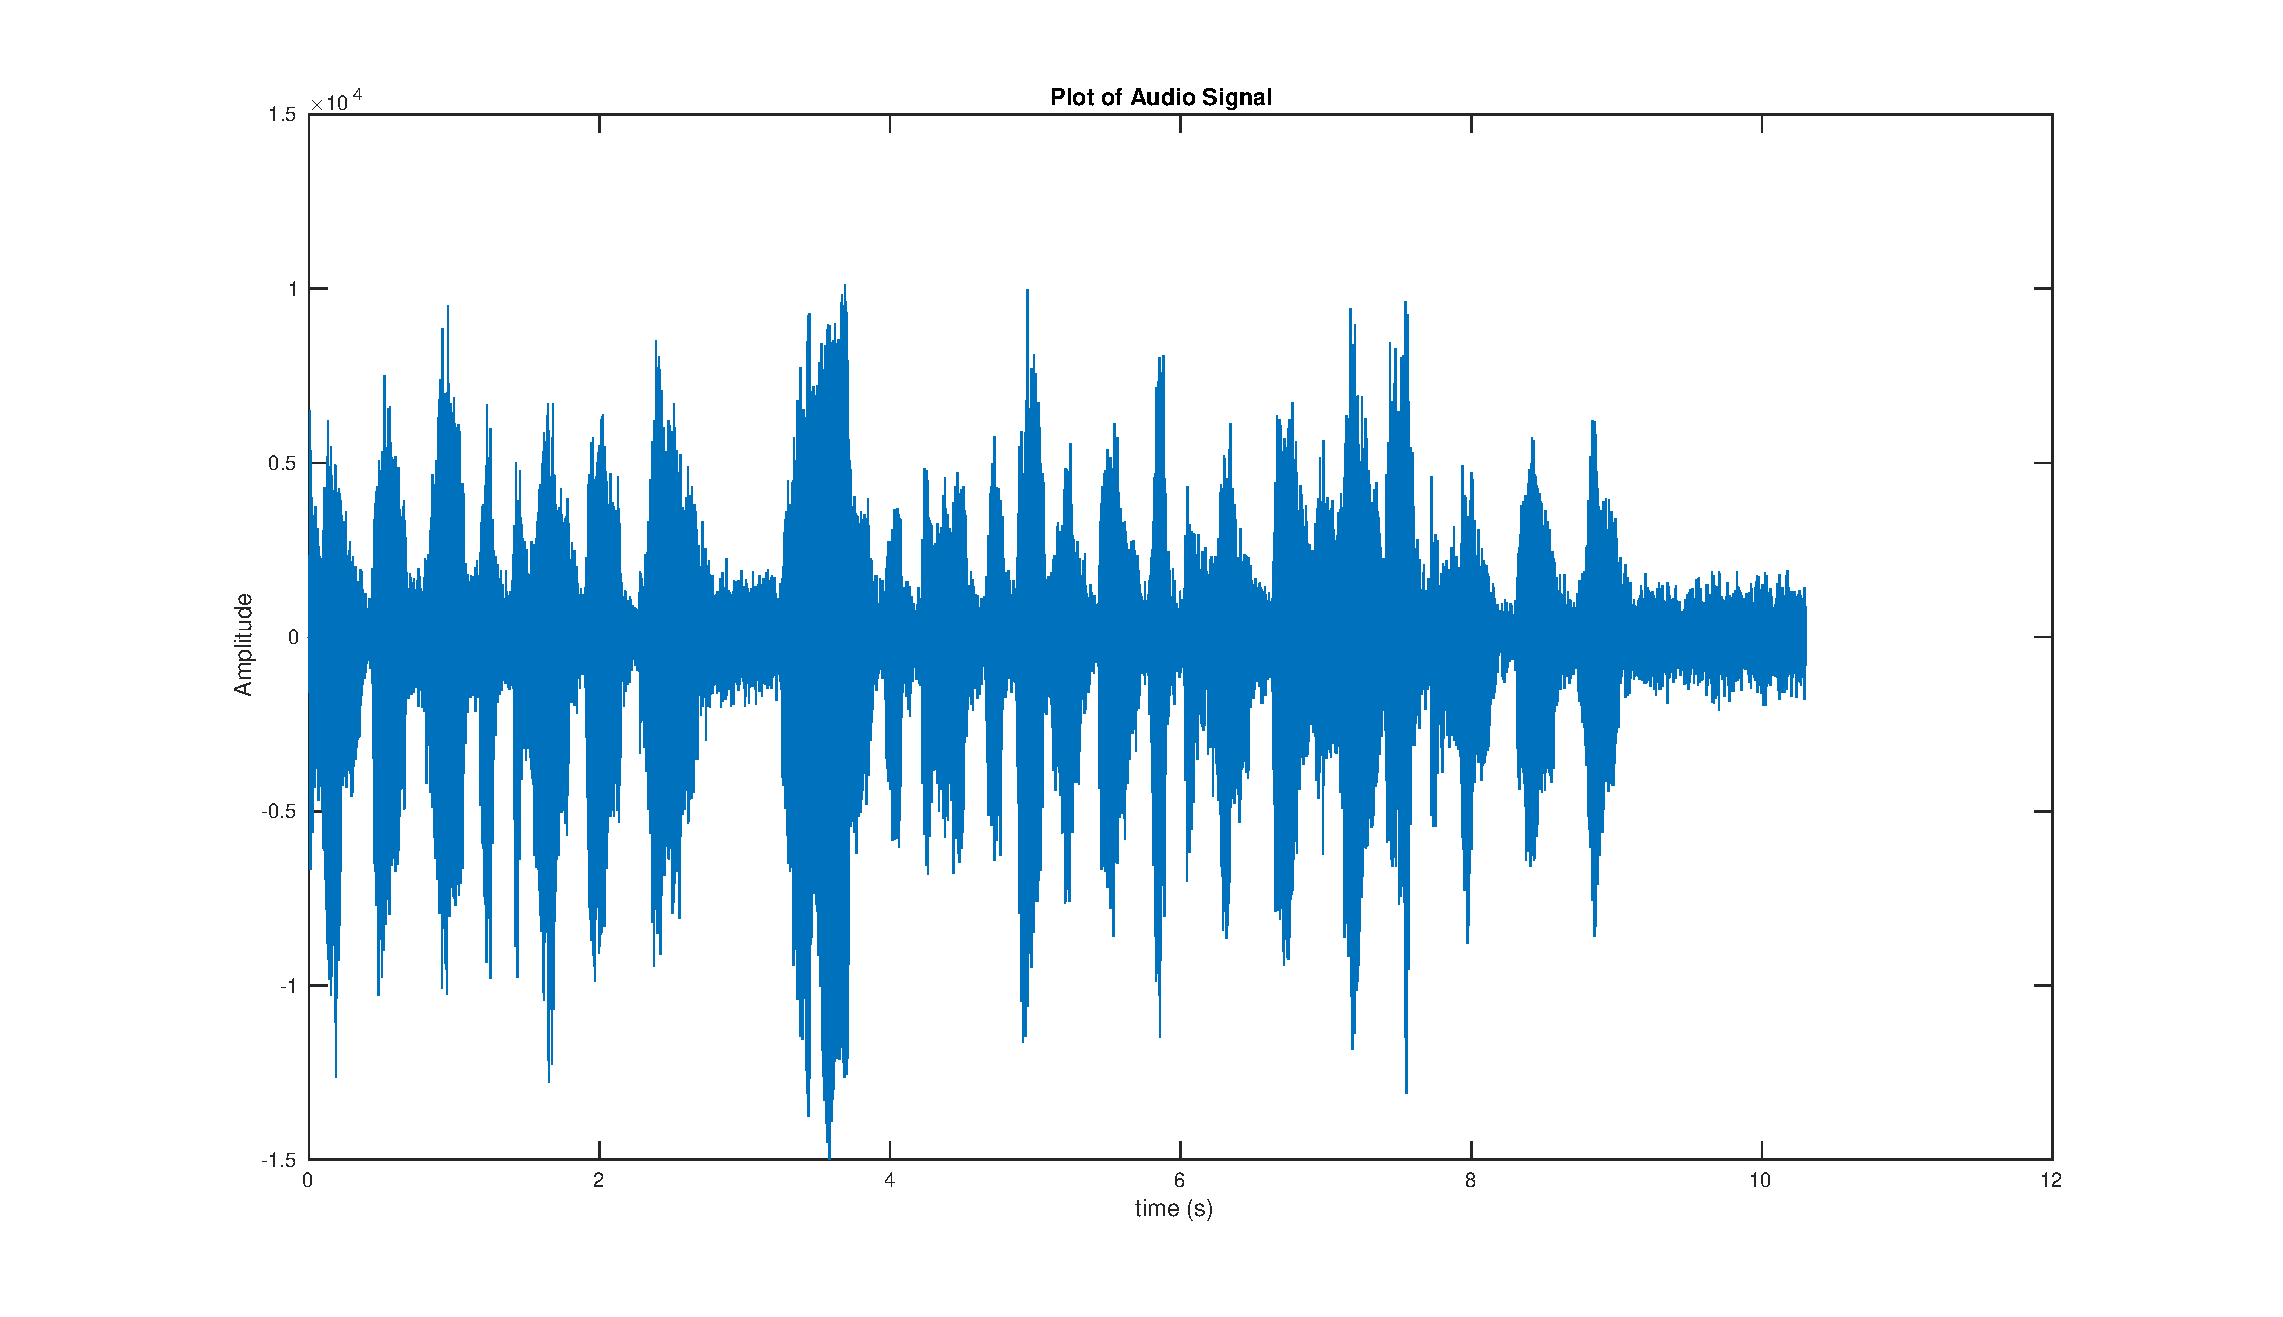
\includegraphics[width=\linewidth]{plot_03}
	\caption{Plot of audio signal sampled at 8kHz.}
	\label{fig: plot_03} 
\end{figure}

\subsubsection{Calculating Global Statistics} 
Calculation of global statistics for both data sets was trivial utilizing built in MATLAB commands. The Google stock trend contain multiple vectors of data, therefore the metrics were computed for each vector. The global statistics for the Google stock trend and the audio signal can be seen in table~1 and 2 below. 


\begin{table}[H] %Google prices
  \centering
    \begin{tabular}{rrrrrr}
    \toprule
    \textbf{Vector} & \textbf{Min} & \textbf{Max} & \textbf{Median} & \textbf{Mean} & \textbf{Variance } \\
    \midrule
    Open  & 49.5  & 612.79 & 265.06 & 286.79 & 16198 \\
    High  & 50.82 & 613.83 & 267.98 & 289.65 & 16345 \\
    Low   & 47.93 & 608.69 & 262.31 & 283.82 & 16030 \\
    Close & 49.95 & 609.47 & 264.83 & 286.74 & 16194 \\
    \bottomrule
    \end{tabular}%
  \caption{Table of global statistics for Google stock trend}
  \label{tab: table_1}
\end{table}%

The global statistics between vectors varied less than ten dollars for minimum, maximum, median, and mean. The variance for stock prices displayed drastic change in comparison. Specifically, the change in variance between the high and low stock prices is 315. 

\begin{table}[H] %Audio Signal
  \centering
    \begin{tabular}{ccccc}
    \toprule
    \textbf{Min} & \textbf{Max} & \textbf{Median} & \textbf{Mean} & \textbf{Variance} \\
    \midrule
    -14993 & 10104 & 83 &  -0.38912   & 4.14E+06 \\
    \bottomrule
    \end{tabular}%
  \caption{Table of global statistics for audio signal}
  \label{tab: table_2}%
\end{table}%

Interesting to note is magnitude and polarity of the mean for the audio signal. The existence of a non-zero mean suggests a DC bias, in this case negative, but its relevance is diminished by the range of values the minimum and maximum  describe. In comparison to range of the signal's medium $(\pm32,767)$ or the actual range of the signal's amplitudes $(10,104 - (- 14,993))$, the mean is essential zero. This is due to an audio signals equal distribution of sample points on the negative and positive axis canceling the sum of amplitudes for the mean calculation. The large swings in amplitude along with the near zero mean, explains the high level of variance in the audio signal compared to the Google stock trend. The calculation for variance is listed below: 
\begin{equation}
\sigma^2 = \frac{1}{N}\sum_{i=1}^{n}(x_i - \bar{x})^2
\end{equation}


\subsubsection{Frame and Windowing}
The frame and windowing technique, covered extensively last semester, consists of splitting the signal into segments called frames. These frames are sized by the number of data points or samples they contain. The number of samples the frame contains is denoted by M. The frame is the increment in which the signal is ``stepped'' through. For each frame in the signal, a window of data is extracted from the signal. A window is a chunk of data points or samples, similar to the frame, centered at the middle of the frame. The number of samples in a window is denoted by N. For this assignment, the mean and variance of each window is taken to represent a frame of data. 

The Google stock prices were run with the following frame and window combinations for the closing prices: N = [7 30] and M = [1 7 14 30]. The plots generated can be seen in figure~\ref{fig: plot_02} below. The frame and window configuration is listed above each subplot as the title. The blue signal is the mean of the window and the red signal is the variance of the window. As the plots describe, the mean of the google stock price is increasing with time. Also can be seen is the variance spiking proportionally with the range between the mean of a window and it's samples.

\begin{figure}[H] %plot google signal frame and windowed 
	\centering 
	\makebox[\textwidth]{\includegraphics[width=8.5in]{plot_02_1}}
	\caption{Plot of Google stock prices filtered via frame and windowing. The blue signal is the mean of the windows. The red signal is the variance of the windows.}
	\label{fig: plot_02} 
\end{figure}

The same process was repeated for the audio signal with the following parameters: M = [40 80 160] N = [160 240]. The plot below in figure~\ref{fig: plot_04} display the results. The blue signal represents the mean of the windows and the black signal represents the variance of the windows. As the plots display, the mean of the windows is magnitudes smaller than the range of the signal's amplitudes calculated from the global statistics. In addition, variance appears to follow the amplitude of the signal which is likely due its similarities to the power calculation of a signal with a near zero mean.

\begin{equation}
x_{rms} = \sqrt{\frac{1}{N}\sum_{i=1}^{n}x_i}
\end{equation} 

\begin{figure}[H] %plot of audio signal frame and windowed 
	\centering 
	\makebox[\textwidth]{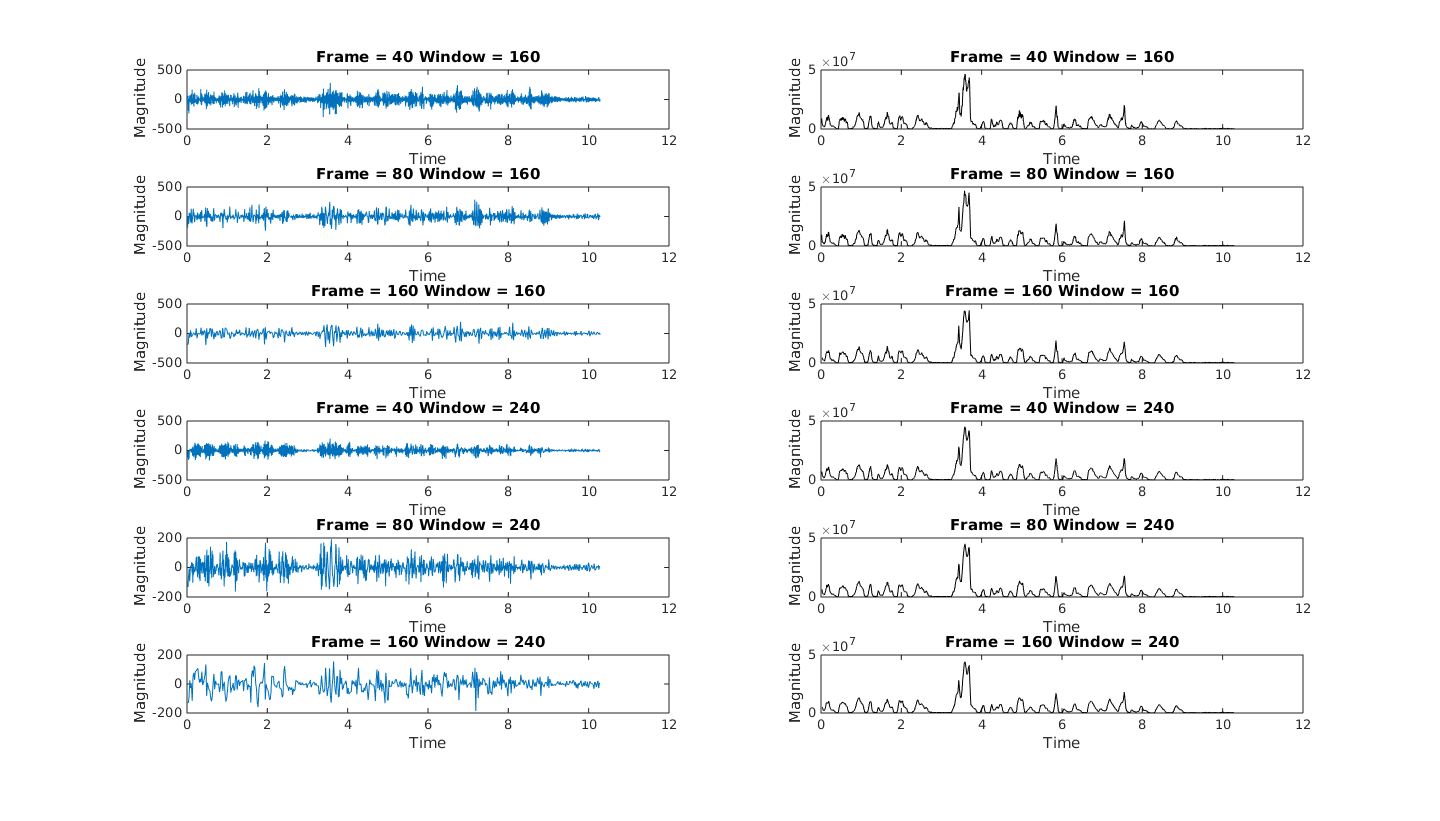
\includegraphics[width=8.5in]{plot_04_}}
	\caption{Plot of audio signal filtered via various frame and window combinations.}
	\label{fig: plot_04} 
\end{figure}

Utilizing the frame and windowing technique permitted the signal to be examined within segments of time, instead of the entire length of the signals existence as with global statistics. For example, the global mean for the Google stock's closing prices was \$286.74, but as all the plots in figure~\ref{fig: plot_02} display, the mean is steadily increasing with time. The global overall mean does not convey if the stock's prices were increasing or decreasing with time. Through the frame and windowed data, the mean was examined through chucks permitting the mean to be displayed for a segment which in turn describes the direction or rate of the signal. This information could be used to predict the future trend of the stock price. 

Frame and windowing the audio signal did not reveal any trends in the mean. The mean did vary through time, but the mean of the windows remained magnitudes smaller compared to the range the signal's amplitudes displayed. This is concurrent with the zero-cross nature of audio signals as previously discussed. Further evidence of this is displayed when the frame size or window size increased to include more sample points, and the mean decreases for each frame. As the number of sample points increase, the mean converges further. 

\section{MATLAB Code} 
%Show and briefly explain your MATLAB code.
The MATLAB code is displayed in listing~1 below. The only peculiarity from the frame and window technique established last semester is the absence of zero stuffing. Zero stuffing would artificially change the mean and variance of a window and therefore any frames with a window which extended past the signal were disregarded. This permitted the windows to be concatenated into a single matrix.
\lstinputlisting[caption=MATLAB code for ca\_01]{../MATLAB/ca_01.m}


\section{Conclusions} 
%Summarize what you found.
Frame and windowing data can introduce another level of information depending upon the signal. Global statistics provided only a singular value to represent the signal for all time while frame and windowing delivers multiple views through segments of time in which rates could be calculated for future prediction. 

How a signal is evaluated is not uniform process. For example, frame and windowing the mean of the audio signal delivered little information due to nature of the medium, but illuminated the Google's average stock price was increasing with time. 

\end{document}
